\begin{figure}[ht]
	\centering
	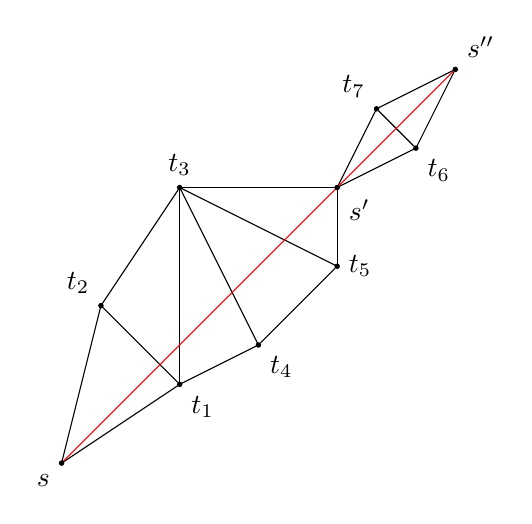
\begin{tikzpicture}[scale=0.5]
		\node[inner sep=0pt, label=below left:\(s\)] (s0) at (0, 0) {};
		\node[inner sep=0pt, label=below right:\(t_1\)] (s1) at (3, 2) {};
		\node[inner sep=0pt, label=above left:\(t_2\)] (s2) at (1, 4) {};
		\node[inner sep=0pt, label=above:\(t_3\)] (s3) at (3, 7) {};
		\node[inner sep=0pt, label=below right:\(t_4\)] (s4) at (5, 3) {};
		\node[inner sep=0pt, label=right:\(t_5\)] (s5) at (7, 5) {};
		\node[inner sep=0pt, label=below right:\(s'\)] (s6) at (7, 7) {};
		\node[inner sep=0pt, label=below right:\(t_6\)] (s7) at (9, 8) {};
		\node[inner sep=0pt, label=above left:\(t_7\)] (s8) at (8, 9) {};
		\node[inner sep=0pt, label=above right:\(s''\)] (s9) at (10, 10) {};

		\draw[color=black] (s0) -- (s1);
		\draw[color=black] (s0) -- (s2);
		\draw[color=black] (s1) -- (s2);
		\draw[color=black] (s1) -- (s3);
		\draw[color=black] (s1) -- (s4);
		\draw[color=black] (s2) -- (s3);
		\draw[color=black] (s3) -- (s4);
		\draw[color=black] (s3) -- (s5);
		\draw[color=black] (s3) -- (s6);
		\draw[color=black] (s4) -- (s5);
		\draw[color=black] (s5) -- (s6);
		\draw[color=black] (s6) -- (s7);
		\draw[color=black] (s6) -- (s8);
		\draw[color=black] (s7) -- (s8);
		\draw[color=black] (s7) -- (s9);
		\draw[color=black] (s8) -- (s9);
		\draw[color=red] (s0) -- (s9);

		\fill[color=black] (s0) circle (2pt);
		\fill[color=black] (s1) circle (2pt);
		\fill[color=black] (s2) circle (2pt);
		\fill[color=black] (s3) circle (2pt);
		\fill[color=black] (s4) circle (2pt);
		\fill[color=black] (s5) circle (2pt);
		\fill[color=black] (s6) circle (2pt);
		\fill[color=black] (s7) circle (2pt);
		\fill[color=black] (s8) circle (2pt);
		\fill[color=black] (s9) circle (2pt);
	\end{tikzpicture}
	\caption{Example unfolded section of a mesh in black with a geodesic between \(s\) and \(s''\) shown in red.}
	\label{fig:geodesic_unfolded_mesh}
\end{figure}

\section{Geodesic Distance}

For this section, due to complexities with the reverse computation, we only have a single variable definition: \begin{center}\begin{tabular}{r|l}
	\(\phi\) & Vector of geodesic distances in \(\mathbb{R}^{\abs{E_G}}\)
\end{tabular}\end{center}

Notation-wise, we will talk about geodesic paths between \(s\) and \(s'\), both in \(E_G\). This actually means we are interested in projecting \(s\) and \(s'\) to the mesh surface, moving them to the nearest mesh vertices, then finding the geodesic path between those two mesh vertices.

\subsection{Forward Computation}
We use \href{https://github.com/zishun/MeshUtility}{MeshUtility}'s implementation of the fast marching method to compute geodesic paths between \(s\) and \(s'\) for every edge \(\cof{s, s'} \in E_G\). This method returns a sequence of vertices and edges the geodesic path passes through, as well as where across the edges the path passes. Automatically, this gives an easy way to compute the geodesic distance.

\subsection{Reverse Computation}
The reverse computation is unfortunately rather complicated and requires some casework. The overall strategy is to first compute the derivative of the geodesic distance between two vertices with respect to the length of any edge in \(E_M\), and then use the chain rule to find the partials we actually want.

To start, a geodesic path is a straight line on an unfolded representation of the mesh, as in Figure~\ref{fig:geodesic_unfolded_mesh}. In fact, we can assign coordinates in \(\mathbb{R}^2\) to the vertices such that the geodesic distance is the Euclidean distance between the start and end points. In the interest of keeping the notation in this section readable, we will use the name of vertices (\(s\), \(t_1\), etc.) to denote these two-dimensional coordinates.

Each geodesic path can be partitioned by the vertices it passes through. If we have the partials of the lengths of each of these segments with respect to each of the mesh's edges, then we automatically have the partials of the length of the entire geodesic simply by addition. In our example, the geodesic path passes through \(s\), \(s'\), and \(s''\). Our analysis below will focus on the segment between \(s\) and \(s'\).

An extremely useful tool is the law of cosines, as well as its derivative. That is, for any three vectors \(u_1\), \(u_2\), and \(u_3\), we have \[\norm{u_2 - u_3}_2^2 = \norm{u_1 - u_2}_2^2 + \norm{u_1 - u_3}_2^2 - 2\pof{u_1 - u_2} \cdot \pof{u_1 - u_3},\] where the last term can be rewritten in terms of the cosine of the angle between \(u_1 - u_2\) and \(u_1 - u_3\).

Define \(M\) to be the length of the distance from \(s\) to \(s'\) (that is, \(M = \norm{s' - s}_2\)), and denote \(\theta_{abc} = m\angle abc\) for any \(a\), \(b\), and \(c\). The partials can be broken into four cases: \begin{itemize}
	\item
	Edges on the boundary. For example, edge \(\cof{t_2, t_3}\). We can then simplify the diagram to Figure~\ref{fig:geodesic_boundary}.

	\begin{figure}[ht]
		\centering
		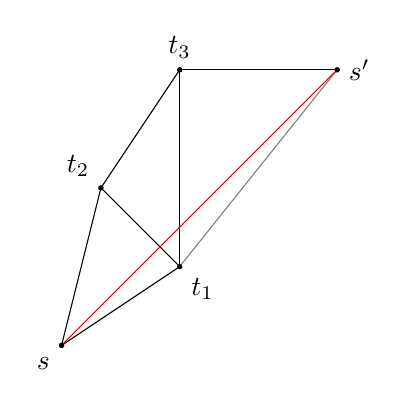
\begin{tikzpicture}[scale=0.5]
			\node[inner sep=0pt, label=below left:\(s\)] (s0) at (0, 0) {};
			\node[inner sep=0pt, label=below right:\(t_1\)] (s1) at (3, 2) {};
			\node[inner sep=0pt, label=above left:\(t_2\)] (s2) at (1, 4) {};
			\node[inner sep=0pt, label=above:\(t_3\)] (s3) at (3, 7) {};
			\node[inner sep=0pt, label=right:\(s'\)] (s6) at (7, 7) {};

			\draw[color=black] (s0) -- (s1);
			\draw[color=black] (s0) -- (s2);
			\draw[color=black] (s1) -- (s2);
			\draw[color=black] (s1) -- (s3);
			\draw[color=gray] (s1) -- (s6);
			\draw[color=black] (s2) -- (s3);
			\draw[color=black] (s3) -- (s6);
			\draw[color=red] (s0) -- (s6);

			\fill[color=black] (s0) circle (2pt);
			\fill[color=black] (s1) circle (2pt);
			\fill[color=black] (s2) circle (2pt);
			\fill[color=black] (s3) circle (2pt);
			\fill[color=black] (s6) circle (2pt);
		\end{tikzpicture}
		\caption{Simplification of Figure~\ref{fig:geodesic_unfolded_mesh} when considering \(\cof{t_2, t_3}\).}
		\label{fig:geodesic_boundary}
	\end{figure}

	Let \(m = \norm{t_2 - t_3}_2\). Applying the law of cosines to \(\angle st_1s'\) and \(\angle t_2t_1t_3\) and differentiating, we have \begin{align*}
		M\frac{\partial M}{\partial m} &= \norm{t_1 - s}_2 \cdot \norm{t_1 - s'}_2 \cdot \sin\pof{\theta_{st_1s'}}\frac{\partial\theta_{st_1s'}}{\partial m}, \\
		m &= \norm{t_1 - t_2}_2 \cdot \norm{t_1 - t_3}_2 \cdot \sin\pof{\theta_{t_2t_1t_3}}\frac{\partial\theta_{t_2t_1t_3}}{\partial m}.
	\end{align*} Now we notice that \(\partial\theta_{st_1s'} / \partial m = \partial\theta_{t_2t_1t_3} / \partial m\), so \[\frac{\partial M}{\partial m} = \frac{\norm{t_2 - t_3}_2 \cdot \norm{\pof{t_1 - s} \times \pof{t_1 - s'}}_2}{\norm{s' - s}_2 \cdot \norm{\pof{t_1 - t_2} \times \pof{t_1 - t_3}}_2}.\]

	\item
	Edges in the interior where the start and end are on ``opposite sides.'' Edge \(\cof{t_1, t_3}\), as shown in Figure~\ref{fig:geodesic_interior_unshared}, exemplifies this case.
	\begin{figure}[ht]
		\centering
		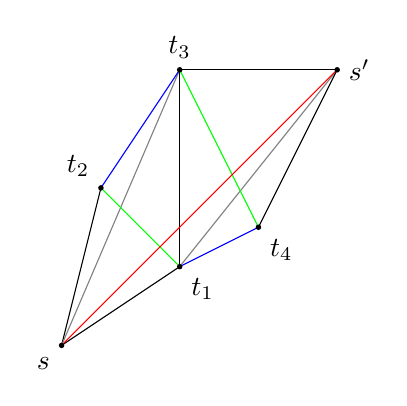
\begin{tikzpicture}[scale=0.5]
			\node[inner sep=0pt, label=below left:\(s\)] (s0) at (0, 0) {};
			\node[inner sep=0pt, label=below right:\(t_1\)] (s1) at (3, 2) {};
			\node[inner sep=0pt, label=above left:\(t_2\)] (s2) at (1, 4) {};
			\node[inner sep=0pt, label=above:\(t_3\)] (s3) at (3, 7) {};
			\node[inner sep=0pt, label=below right:\(t_4\)] (s4) at (5, 3) {};
			\node[inner sep=0pt, label=right:\(s'\)] (s6) at (7, 7) {};

			\draw[color=black] (s0) -- (s1);
			\draw[color=black] (s0) -- (s2);
			\draw[color=gray] (s0) -- (s3);
			\draw[color=green] (s1) -- (s2);
			\draw[color=black] (s1) -- (s3);
			\draw[color=blue] (s1) -- (s4);
			\draw[color=gray] (s1) -- (s6);
			\draw[color=blue] (s2) -- (s3);
			\draw[color=green] (s3) -- (s4);
			\draw[color=black] (s3) -- (s6);
			\draw[color=black] (s4) -- (s6);
			\draw[color=red] (s0) -- (s6);

			\fill[color=black] (s0) circle (2pt);
			\fill[color=black] (s1) circle (2pt);
			\fill[color=black] (s2) circle (2pt);
			\fill[color=black] (s3) circle (2pt);
			\fill[color=black] (s4) circle (2pt);
			\fill[color=black] (s6) circle (2pt);
		\end{tikzpicture}
		\caption{Simplification of Figure~\ref{fig:geodesic_unfolded_mesh} when considering \(\cof{t_1, t_3}\). Note that the triangles \(\triangle st_1t_2\) and \(\triangle s't_3t_4\) are connected to opposite sides of the quadrilateral \(\square t_1t_4t_3t_2\). Alternatively, the two triangles share no vertices.}
		\label{fig:geodesic_interior_unshared}
	\end{figure}

	The computation here is unfortunately complex, but the idea is similar to that of the previous case. Let \(m = \norm{t_1 - t_3}_2\). We first apply the law of cosines to \(\angle t_3t_2t_1\), and \(\angle t_3t_2s\). Then we differentiate each result. This yields \begin{align*}
		\frac{\partial\theta_{t_3t_2t_1}}{\partial m} &= \frac{\norm{t_3 - t_1}_2}{\norm{\pof{t_2 - t_1} \times \pof{t_2 - t_3}}_2}, \\
		\frac{\partial\norm{t_3 - s}_2}{\partial m} &= \frac{\norm{\pof{t_2 - s} \times \pof{t_2 - t_3}}_2}{\norm{t_3 - s}_2} \cdot \frac{\partial\theta_{t_3t_2s}}{\partial m}. \\
		\intertext{Noting that \(\partial\theta_{t_3t_2s} / \partial m\) and \(\partial\theta_{t_3t_2t_1} / \partial m\) are equivalent, we obtain.}
		\frac{\partial\norm{t_3 - s}_2}{\partial m} &= \frac{\norm{t_3 - t_1}_2 \cdot \norm{\pof{t_2 - s} \times \pof{t_2 - t_3}}_2}{\norm{t_3 - s}_2 \cdot \norm{\pof{t_2 - t_1} \times \pof{t_2 - t_3}}_2}. \\
		\intertext{Similarly,}
		\frac{\partial\norm{t_1 - s'}_2}{\partial m} &= \frac{\norm{t_1 - t_3}_2 \cdot \norm{\pof{t_4 - s'} \times \pof{t_4 - t_1}}_2}{\norm{t_1 - s'}_2 \cdot \norm{\pof{t_4 - t_3} \times \pof{t_4 - t_1}}_2}.
	\end{align*}

	Now we apply the law of cosines to \(\angle st_1s'\) and differentiate. This yields \begin{align*}
		\norm{s' - s}_2\frac{\partial M}{\partial m} &= \norm{t_1 - s'}_2 \cdot \frac{\partial\norm{t_1 - s'}_2}{\partial m} - \frac{\pof{t_1 - s} \cdot \pof{t_1 - s'}}{\norm{t_1 - s'}_2} \cdot \frac{\partial\norm{t_1 - s'}_2}{\partial m} \\
		&\qquad + \norm{\pof{t_1 - s} \times \pof{t_1 - s'}}_2 \cdot \frac{\partial\theta_{st_1s'}}{\partial m} \\
		&= \pof{1 - \frac{\pof{t_1 - s} \cdot \pof{t_1 - s'}}{\norm{t_1 - s'}_2^2}} \cdot \frac{\norm{t_1 - t_3}_2 \cdot \norm{\pof{t_4 - s'} \times \pof{t_4 - t_1}}_2}{\norm{\pof{t_4 - t_3} \times \pof{t_4 - t_1}}_2} \\
		&\qquad+ \norm{\pof{t_1 - s} \times \pof{t_1 - s'}}_2 \cdot \frac{\partial\theta_{st_1s'}}{\partial m}. \\
		\intertext{Applying the same process to \(\angle t_1s't_3\), \(\angle s't_3s\), and \(\angle t_3st_1\), we get}
		\norm{t_1 - t_3}_2 &= \pof{1 - \frac{\pof{t_3 - s'} \cdot \pof{t_1 - s'}}{\norm{t_1 - s'}_2^2}} \cdot \frac{\norm{t_1 - t_3}_2 \cdot \norm{\pof{t_4 - s'} \times \pof{t_4 - t_1}}_2}{\norm{\pof{t_4 - t_3} \times \pof{t_4 - t_1}}_2} \\
		&\qquad+ \norm{\pof{t_1 - s'} \times \pof{t_3 - s'}}_2 \cdot \frac{\partial\theta_{t_1s't_3}}{\partial m}, \\
		\norm{s' - s}_2\frac{\partial M}{\partial m} &= \pof{1 - \frac{\pof{t_3 - s} \cdot \pof{t_3 - s'}}{\norm{t_3 - s'}_2^2}} \cdot \frac{\norm{t_1 - t_3}_2 \cdot \norm{\pof{t_2 - s} \times \pof{t_2 - t_3}}_2}{\norm{\pof{t_2 - t_1} \times \pof{t_2 - t_3}}_2} \\
		&\qquad+ \norm{\pof{t_3 - s} \times \pof{t_3 - s'}}_2 \cdot \frac{\partial\theta_{s't_3s}}{\partial m}, \\
		\intertext{and}
		\norm{t_1 - t_3}_2 &= \pof{1 - \frac{\pof{t_1 - s'} \cdot \pof{t_3 - s'}}{\norm{t_3 - s'}_2^2}} \cdot \frac{\norm{t_1 - t_3}_2 \cdot \norm{\pof{t_2 - s} \times \pof{t_2 - t_3}}_2}{\norm{\pof{t_2 - t_1} \times \pof{t_2 - t_3}}_2} \\
		&\qquad+ \norm{\pof{t_1 - s} \times \pof{t_3 - s}}_2 \cdot \frac{\partial\theta_{t_3st_1}}{\partial m}.
	\end{align*}

	We now recognize \begin{align*}
		\frac{\partial\theta_{st_1s'}}{\partial m} + \frac{\partial\theta_{t_1s't_3}}{\partial m} + \frac{\partial\theta_{s't_3s}}{\partial m} + \frac{\partial\theta_{t_3st_1}}{\partial m} &= \frac{\partial}{\partial m}\pof{\theta_{st_1s'} + \theta_{t_1s't_3} + \theta_{s't_3s} + \theta_{t_3st_1}} \\
			&= \frac{\partial}{\partial m}\pof{2\pi} \\
			&= 0.
	\end{align*} We can thus combine the last four law of cosine computations and cancel out all of the unknown derivatives except \(\partial M / \partial m\). The final result is rather complicated expression. Due to formatting issues, it will be presented in two parts: the numerator and denominator of a fraction. The numerator is \begin{align*}
		&\hspace{-2em}\pof{1 - \frac{\pof{t_1 - s} \cdot \pof{t_1 - s'}}{\norm{t_1 - s'}_2^2}} \cdot \frac{\norm{t_1 - t_3}_2 \cdot \norm{\pof{t_4 - s'} \times \pof{t_4 - t_1}}_2}{\norm{\pof{t_4 - t_3} \times \pof{t_4 - t_1}}_2 \cdot \norm{\pof{t_1 - s} \times \pof{t_1 - s'}}_2} \\
		&+ \pof{1 - \frac{\pof{t_3 - s'} \cdot \pof{t_1 - s'}}{\norm{t_1 - s'}_2^2}} \cdot \frac{\norm{t_1 - t_3}_2 \cdot \norm{\pof{t_4 - s'} \times \pof{t_4 - t_1}}_2}{\norm{\pof{t_4 - t_3} \times \pof{t_4 - t_1}}_2 \cdot \norm{\pof{t_1 - s'} \times \pof{t_3 - s'}}_2} \\
		&+ \pof{1 - \frac{\pof{t_3 - s} \cdot \pof{t_3 - s'}}{\norm{t_3 - s'}_2^2}} \cdot \frac{\norm{t_1 - t_3}_2 \cdot \norm{\pof{t_2 - s} \times \pof{t_2 - t_3}}_2}{\norm{\pof{t_2 - t_1} \times \pof{t_2 - t_3}}_2 \cdot \norm{\pof{t_3 - s} \times \pof{t_3 - s'}}_2} \\
		&+ \pof{1 - \frac{\pof{t_1 - s'} \cdot \pof{t_3 - s'}}{\norm{t_3 - s'}_2^2}} \cdot \frac{\norm{t_1 - t_3}_2 \cdot \norm{\pof{t_2 - s} \times \pof{t_2 - t_3}}_2}{\norm{\pof{t_2 - t_1} \times \pof{t_2 - t_3}}_2 \cdot \norm{\pof{t_1 - s} \times \pof{t_3 - s}}_2} \\
		&- \frac{\norm{t_1 - t_3}_2}{\norm{\pof{t_1 - s'} \times \pof{t_3 - s'}}_2} - \frac{\norm{t_1 - t_3}_2}{\norm{\pof{t_1 - s} \times \pof{t_3 - s}}_2}.
	\end{align*} and the denominator is \[\frac{\norm{s' - s}_2}{\norm{\pof{t_1 - s} \times \pof{t_1 - s'}}_2} + \frac{\norm{s' - s}_2}{\norm{\pof{t_3 - s} \times \pof{t_3 - s'}}_2}.\]

	\item
	Edges in the interior where the start and end are on the ``same side.'' In our example, edge \(\cof{t_3, t_4}\) satisfies this, shown in Figure~\ref{fig:geodesic_interior_shared}.

	\begin{figure}[ht]
		\centering
		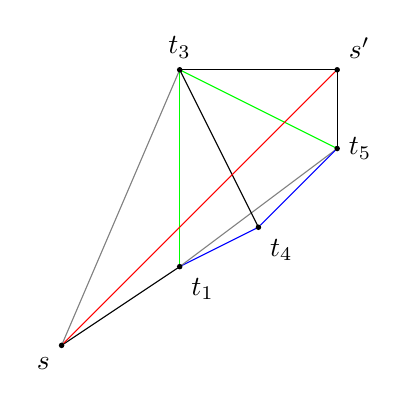
\begin{tikzpicture}[scale=0.5]
			\node[inner sep=0pt, label=below left:\(s\)] (s0) at (0, 0) {};
			\node[inner sep=0pt, label=below right:\(t_1\)] (s1) at (3, 2) {};
			\node[inner sep=0pt, label=above:\(t_3\)] (s3) at (3, 7) {};
			\node[inner sep=0pt, label=below right:\(t_4\)] (s4) at (5, 3) {};
			\node[inner sep=0pt, label=right:\(t_5\)] (s5) at (7, 5) {};
			\node[inner sep=0pt, label=above right:\(s'\)] (s6) at (7, 7) {};

			\draw[color=black] (s0) -- (s1);
			\draw[color=gray] (s0) -- (s3);
			\draw[color=green] (s1) -- (s3);
			\draw[color=blue] (s1) -- (s4);
			\draw[color=gray] (s1) -- (s5);
			\draw[color=black] (s3) -- (s4);
			\draw[color=green] (s3) -- (s5);
			\draw[color=black] (s3) -- (s6);
			\draw[color=blue] (s4) -- (s5);
			\draw[color=black] (s5) -- (s6);
			\draw[color=red] (s0) -- (s6);

			\fill[color=black] (s0) circle (2pt);
			\fill[color=black] (s1) circle (2pt);
			\fill[color=black] (s3) circle (2pt);
			\fill[color=black] (s4) circle (2pt);
			\fill[color=black] (s5) circle (2pt);
			\fill[color=black] (s6) circle (2pt);
		\end{tikzpicture}
		\caption{Simplification of Figure~\ref{fig:geodesic_unfolded_mesh} when considering \(\cof{t_3, t_4}\). Note that the triangles \(\triangle st_1t_3\) and \(\triangle s't_3t_5\) are connected to adjacent sides of the quadrilateral \(\square t_1t_4t_5t_3\). Alternatively, the two triangles share the vertex \(t_3\).}
		\label{fig:geodesic_interior_shared}
	\end{figure}

	Let \(m = \norm{t_3 - t_4}_2\) and \(q = \norm{t_1 - t_5}_2\). Once again, the strategy is to use the law of cosines and differentiate. Using the angles \(\angle t_1t_4t_5\), \(\angle t_4t_5t_3\), \(\angle t_5t_3t_1\), and \(t_3t_1t_4\), we get \begin{align*}
		\norm{t_1 - t_5}_2\frac{\partial q}{\partial m} &= \norm{\pof{t_4 - t_1} \times \pof{t_4 - t_5}}_2 \cdot \frac{\partial\theta_{t_1t_4t_5}}{\partial m}, \\
		\norm{t_3 - t_4}_2 &= \norm{\pof{t_5 - t_3} \times \pof{t_5 - t_4}}_2 \cdot \frac{\partial\theta_{t_4t_5t_3}}{\partial m}, \\
		\norm{t_1 - t_5}_2\frac{\partial q}{\partial m} &= \norm{\pof{t_3 - t_1} \times \pof{t_3 - t_5}}_2 \cdot \frac{\partial\theta_{t_5t_3t_1}}{\partial m}, \\
		\norm{t_3 - t_4}_2 &= \norm{\pof{t_1 - t_3} \times \pof{t_1 - t_4}}_2 \cdot \frac{\partial\theta_{t_3t_1t_4}}{\partial m}.
	\end{align*} We now again apply the trick where the sum of the angle is constant \(2\pi\), meaning the sum of the partials is \(0\). Scaling the equations, adding them, and solving, we get \[\frac{\partial q}{\partial m} = -\frac{\norm{t_3 - t_4}_2 \cdot \pof{\frac{1}{\norm{\pof{t_5 - t_3} \times \pof{t_5 - t_4}}_2} + \frac{1}{\norm{\pof{t_1 - t_3} \times \pof{t_1 - t_4}}_2}}}{\norm{t_1 - t_5}_2 \cdot \pof{\frac{1}{\norm{\pof{t_4 - t_1} \times \pof{t_4 - t_5}}_2} + \frac{1}{\norm{\pof{t_3 - t_1} \times \pof{t_3 - t_5}}_2}}}.\]

	We finish this case by noting \[\frac{\dif M}{\dif q} = \frac{\norm{t_1 - t_5}_2 \cdot \norm{\pof{t_3 - s} \times \pof{t_3 - s'}}_2}{\norm{s - s'}_2 \cdot \norm{\pof{t_3 - t_1} \times \pof{t_3 - t_5}}_2}.\] From the chain rule, we thus have \[\frac{\partial M}{\partial m} = -\frac{\norm{t_3 - t_4}_2 \cdot \norm{\pof{t_3 - s} \times \pof{t_3 - s'}}_2 \cdot \pof{\frac{1}{\norm{\pof{t_5 - t_3} \times \pof{t_5 - t_4}}_2} + \frac{1}{\norm{\pof{t_1 - t_3} \times \pof{t_1 - t_4}}_2}}}{\norm{s - s'}_2 \cdot \pof{\frac{\norm{\pof{t_3 - t_1} \times \pof{t_3 - t_5}}_2}{\norm{\pof{t_4 - t_1} \times \pof{t_4 - t_5}}_2} + 1}}.\]

	\item
	Edges not incident to faces through which the geodesic path passes. The lengths of these edges have no effect on the length of the geodesic path (locally speaking, at least), so the partials here are \(0\).
\end{itemize}

One might think that there is a fifth case missing from the above analysis. In particular, cases similar to that seen in Figure~\ref{fig:geodesic_degenerate} aren't immediately similar to any of the situations referenced above. However, if we make the identifications \begin{align*}
	s &\leftarrow s' & t_1 &\leftarrow s' & t_3 &\leftarrow t_7 \\
	t_4 &\leftarrow t_6 & t_5 &\leftarrow s'' & s' &\leftarrow s'',
\end{align*} we see that Figure~\ref{fig:geodesic_degenerate} is just a degenerate instance of Figure~\ref{fig:geodesic_interior_shared}.

\begin{figure}[ht]
	\centering
	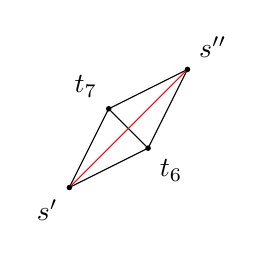
\begin{tikzpicture}[scale=0.5]
		\node[inner sep=0pt, label=below left:\(s'\)] (s6) at (7, 7) {};
		\node[inner sep=0pt, label=below right:\(t_6\)] (s7) at (9, 8) {};
		\node[inner sep=0pt, label=above left:\(t_7\)] (s8) at (8, 9) {};
		\node[inner sep=0pt, label=above right:\(s''\)] (s9) at (10, 10) {};

		\draw[color=black] (s6) -- (s7);
		\draw[color=black] (s6) -- (s8);
		\draw[color=black] (s7) -- (s8);
		\draw[color=black] (s7) -- (s9);
		\draw[color=black] (s8) -- (s9);
		\draw[color=red] (s6) -- (s9);

		\fill[color=black] (s6) circle (2pt);
		\fill[color=black] (s7) circle (2pt);
		\fill[color=black] (s8) circle (2pt);
		\fill[color=black] (s9) circle (2pt);
	\end{tikzpicture}
	\caption{Simplification of Figure~\ref{fig:geodesic_unfolded_mesh} when considering \(\cof{t_6, t_7}\).}
	\label{fig:geodesic_degenerate}
\end{figure}

With the partials of the geodesic distances with respect to the length of the edges of the mesh in hand, we need only compute the partials of the edge lengths with respect to the mesh parameters. We find \[\frac{\partial\norm{v_i - v_j}_2}{\partial z_\ell} = \begin{cases}
	\frac{v_i - v_j}{\norm{v_i - v_j}_2} \cdot \frac{\partial v_\ell}{\partial z_\ell} & \text{if \(\ell = i\),} \\
	\frac{v_j - v_i}{\norm{v_i - v_j}_2} \cdot \frac{\partial v_\ell}{\partial z_\ell} & \text{if \(\ell = j\),} \\
	0 & \text{otherwise.}
\end{cases}\] All that remains is to use the chain rule to compute the partials of the geodesic distance with respect to the mesh parameters.
